\subsection{Pré-traitement}
On regarde le nombre de \texttt{\#}, \texttt{@} et lien par tweet selon le type de tweet scientifique (\autoref{fig:hashtag_count}).

\begin{figure}[H]
    \centering
    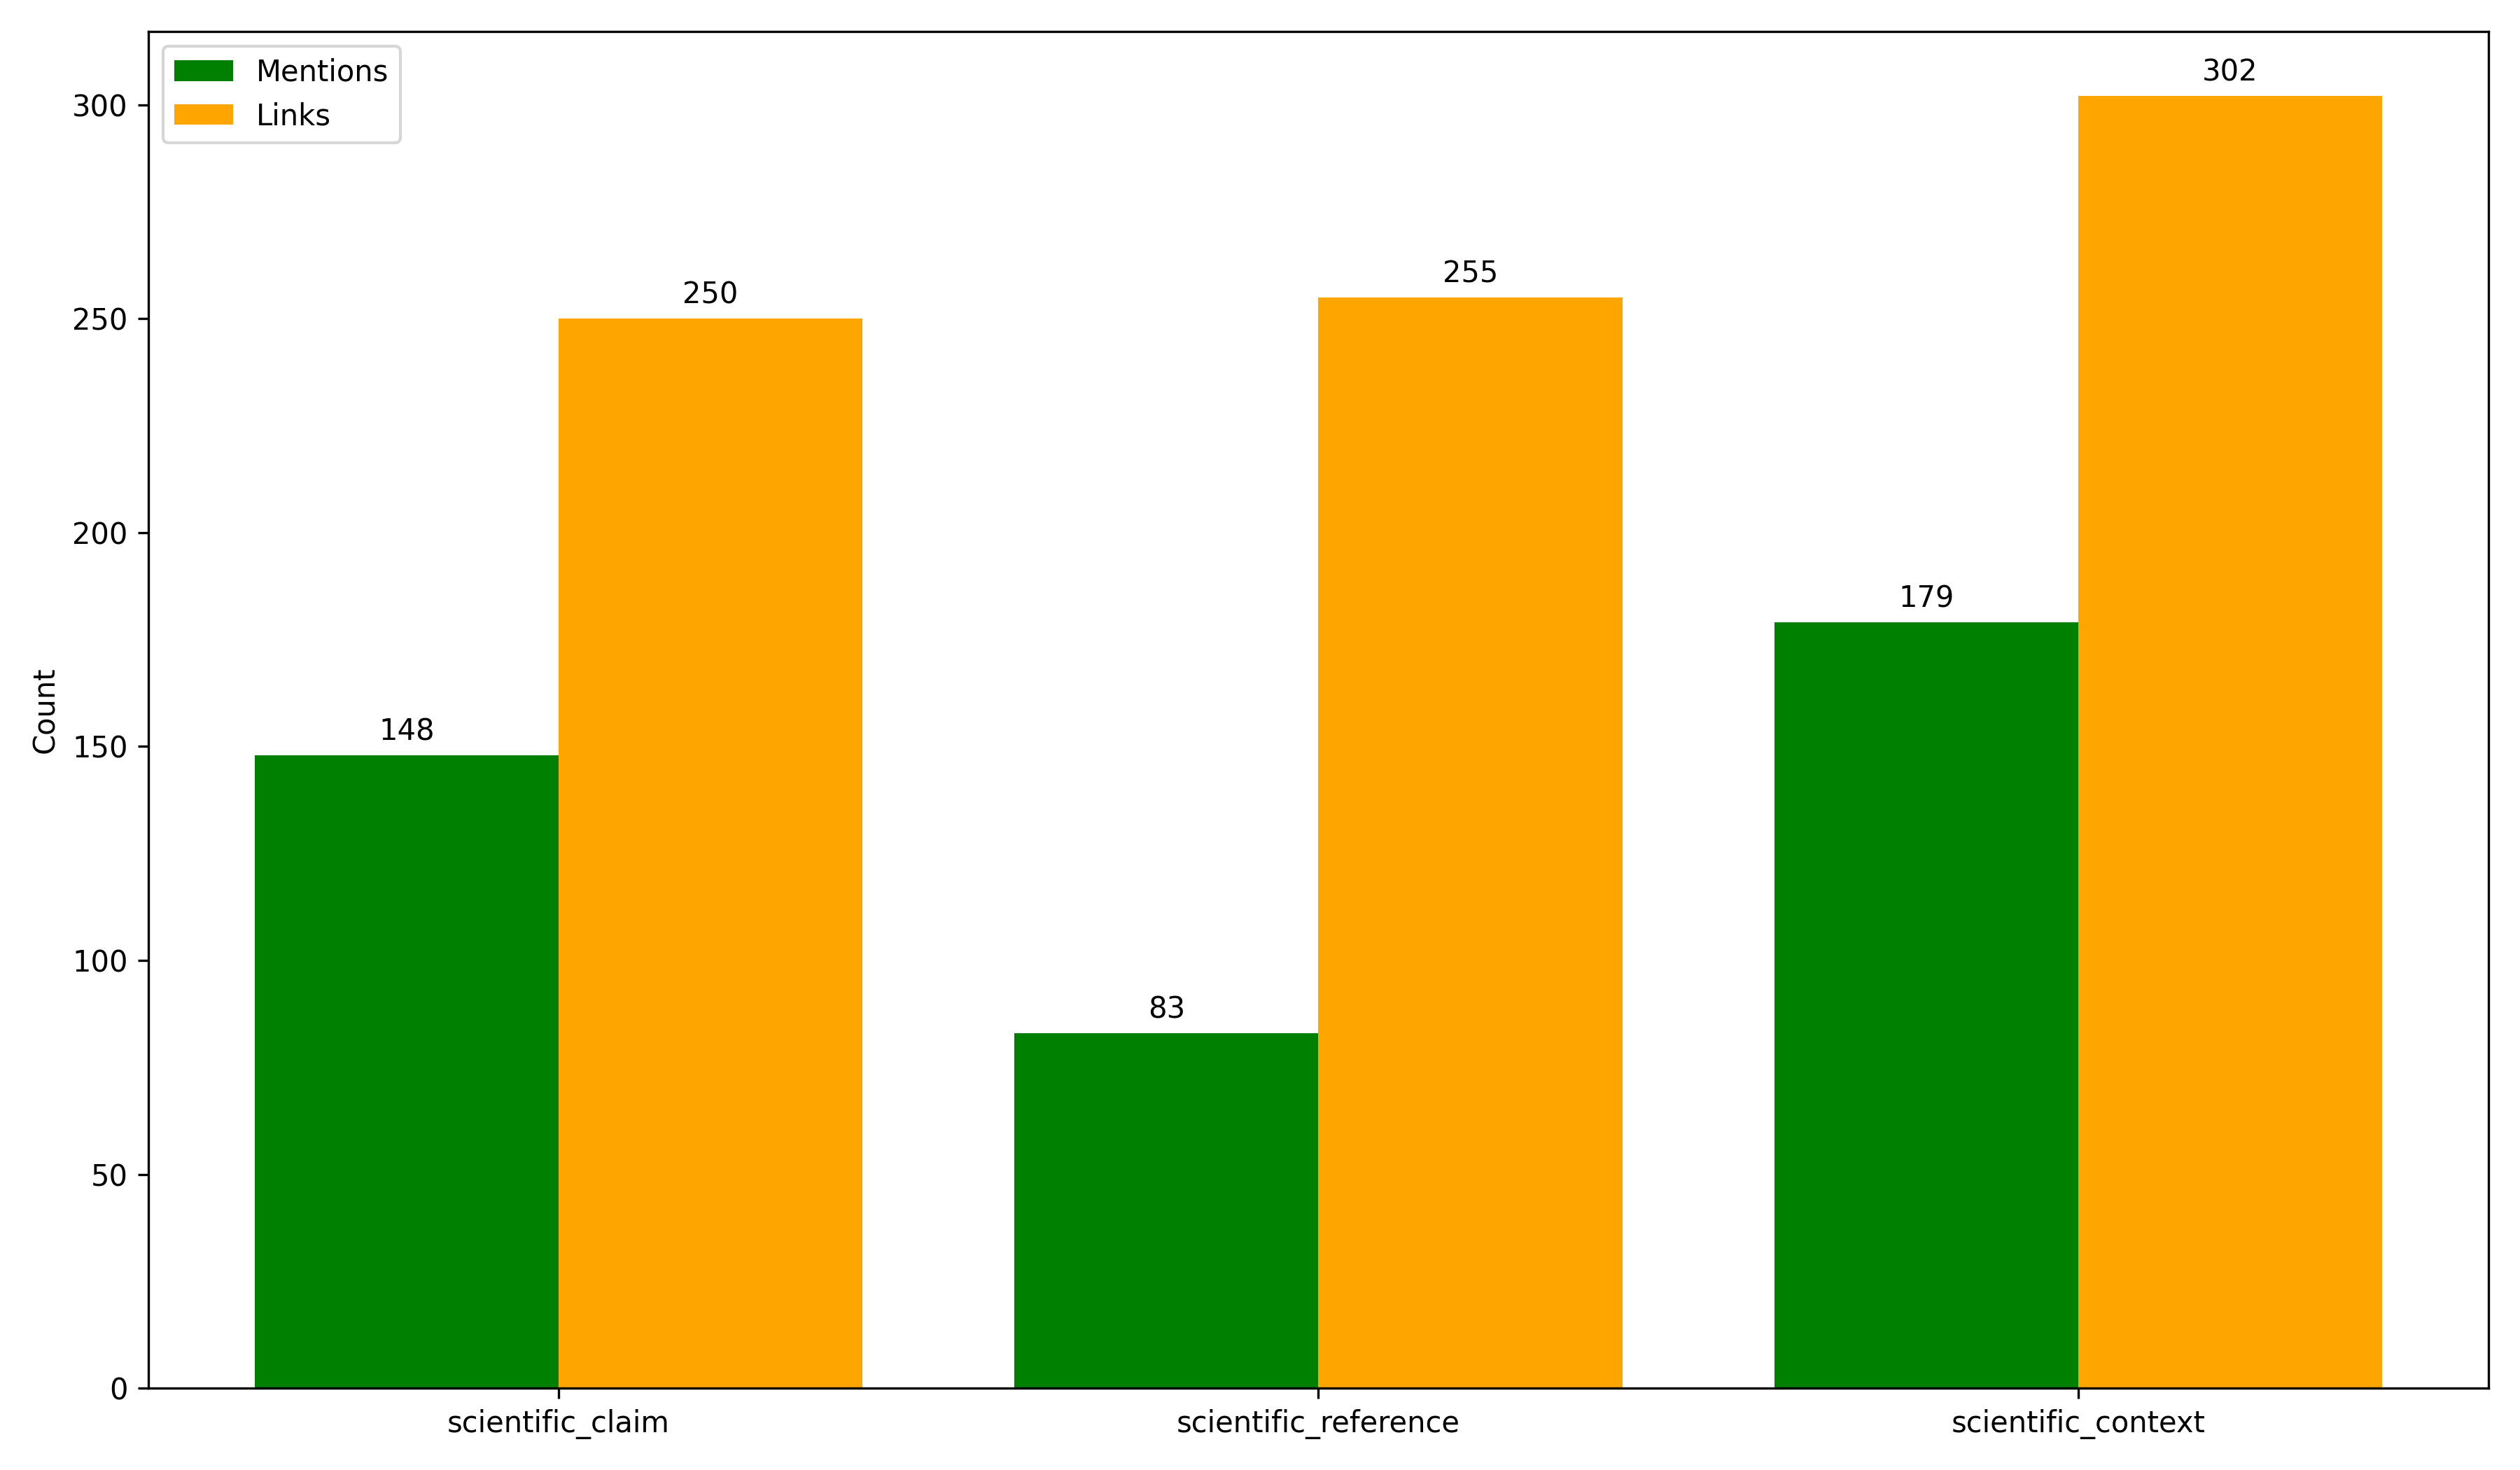
\includegraphics[width=1\textwidth]{images/hashtag_links_mentions_count_outliers}
    \caption{Nombre de hashtags par tweet selon le type de tweet scientifique.}
    \label{fig:hashtag_count}
\end{figure}

Après avoir réalisé des tests d'indépendance de student sur chaque variable, les \textit{p-values} ne descendent pas en dessous de 0.18 donc on ne remarque pas de différence significative entre les tweets scientifiques et non scientifiques.
On peut ainsi conclure que ces variables ne sont pas pertinentes pour la classification des tweets scientifiques, on les retirera de notre dataset.
Malgrès tout, les \texttt{\#} permettent une meilleur accuracy overall, on l'a donc gardé.

\subsection{Modélisation}
Pour chacunes des étapes, nous allons comparer différents modèles entre eux pour sélectionner le meilleur modèle.
Par meilleur modèle, on entend la meilleure précision et le plus petit écart-type.

Chaque modèle est testé par cross-validation sur 10 itérations.

\subsection{Modèle 1: Sci vs Non-sci}

\begin{figure}[H]
    \centering
    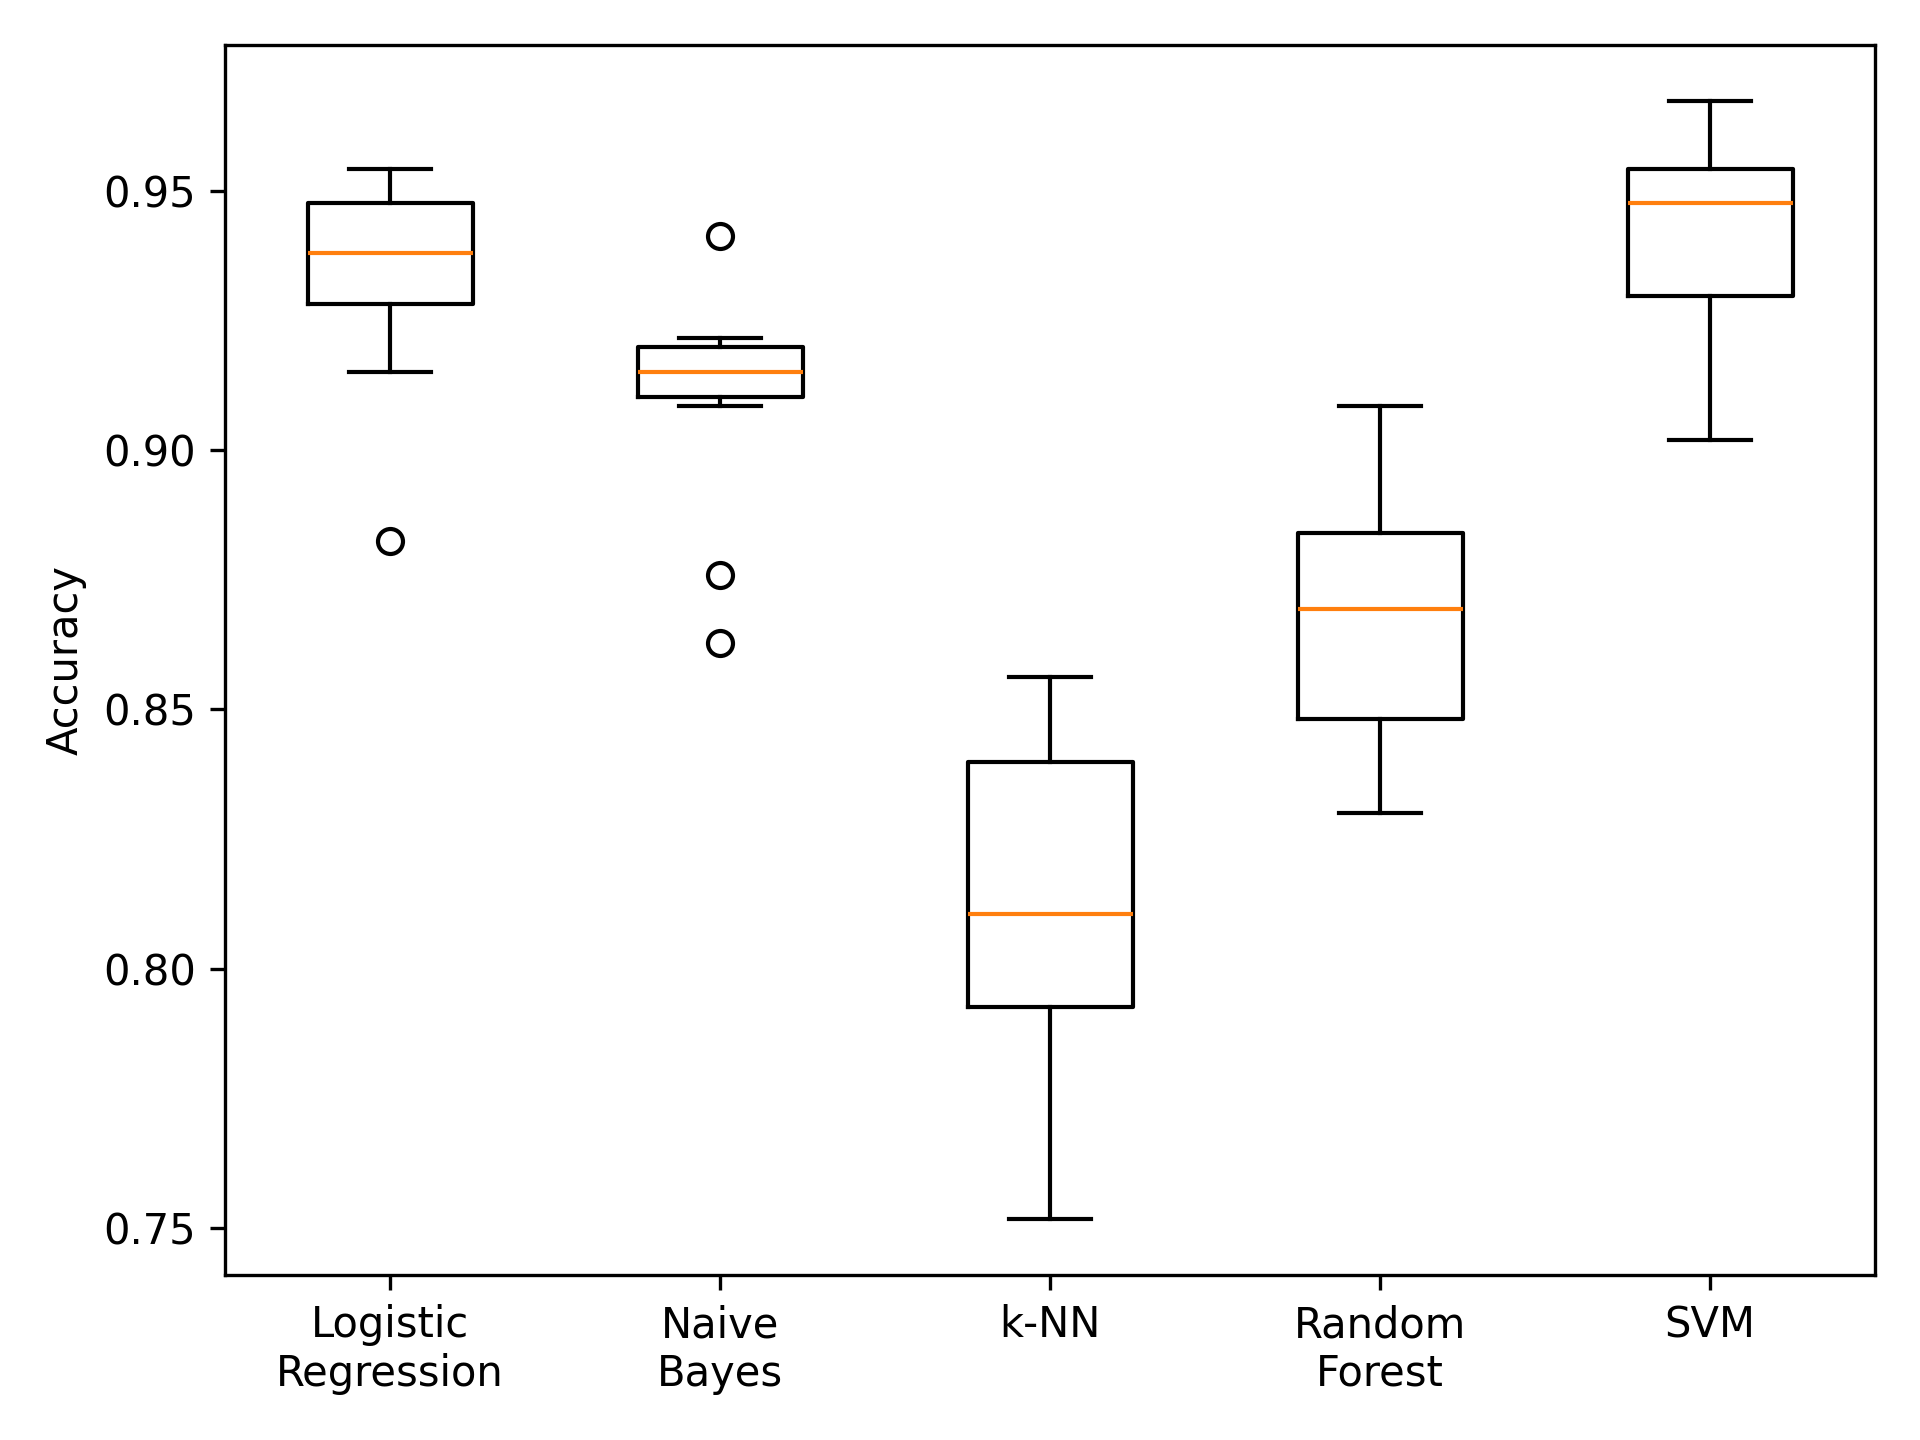
\includegraphics{images/model_comparison}
    \caption{Comparaison des modèles pour la classification des tweets scientifiques et non scientifiques.}
    \label{fig:model_comparison_sci_nsci}
\end{figure}

Les deux meilleurs modèles sont le \texttt{SVM} et \texttt{Logistic Regression} mais on préfèrera cette dernière, car elle a un plus petit écart-type.

\subsection{Modèle 2: claim et ref vs contexte}

\subsection{Modèle 3: claim vs ref vs contexte}
